%%%%%%%%%%%%%%%%%%%%%%%%%%%%%%%%%%%%%%%%%
% Important note:
% Chapter heading images should have a 2:1 width:height ratio,
% e.g. 920px width and 460px height.
%
% The original template (the Legrand Orange Book Template) can be found here --> http://www.latextemplates.com/template/the-legrand-orange-book
%
% Original author of the Legrand Orange Book Template:
% Mathias Legrand (legrand.mathias@gmail.com) with modifications by:
% Vel (vel@latextemplates.com)
%
% Original License:
% CC BY-NC-SA 3.0 (http://creativecommons.org/licenses/by-nc-sa/3.0/)
%%%%%%%%%%%%%%%%%%%%%%%%%%%%%%%%%%%%%%%%%
 
%----------------------------------------------------------------------------------------
%	PACKAGES AND OTHER DOCUMENT CONFIGURATIONS
%----------------------------------------------------------------------------------------

\documentclass[11pt,fleqn]{book} % Default font size and left-justified equations

\usepackage[top=3cm,bottom=3cm,left=3.2cm,right=3.2cm,headsep=10pt,letterpaper]{geometry} % Page margins

\usepackage{xcolor} % Required for specifying colors by name
\definecolor{ocre}{RGB}{52,177,201} % Define the orange color used for highlighting throughout the book

% Font Settings
\usepackage{avant} % Use the Avantgarde font for headings
%\usepackage{times} % Use the Times font for headings
\usepackage{mathptmx} % Use the Adobe Times Roman as the default text font together with math symbols from the Sym­bol, Chancery and Com­puter Modern fonts

\usepackage{microtype} % Slightly tweak font spacing for aesthetics
\usepackage[utf8]{inputenc} % Required for including letters with accents
\usepackage[T1]{fontenc} % Use 8-bit encoding that has 256 glyphs

\usepackage{csquotes}

% Bibliography
\usepackage[style=alphabetic,sorting=nyt,sortcites=true,autopunct=true,babel=hyphen,hyperref=true,abbreviate=false,backref=true,backend=biber]{biblatex}
\addbibresource{bibliography.bib} % BibTeX bibliography file
\defbibheading{bibempty}{}

%%%%%%%%%%%%%%%%%%%%%%%%%%%%%%%%%%%%%%%%%
% This is based on the Legrand Orange Book
% Structural Definitions File
%
% The original template (the Legrand Orange Book Template) can be found here --> http://www.latextemplates.com/template/the-legrand-orange-book
%
% Original author of the Legrand Orange Book Template::
% Mathias Legrand (legrand.mathias@gmail.com) with modifications by:
% Vel (vel@latextemplates.com)
%
% Original License:
% CC BY-NC-SA 3.0 (http://creativecommons.org/licenses/by-nc-sa/3.0/)
%
%%%%%%%%%%%%%%%%%%%%%%%%%%%%%%%%%%%%%%%%%
%----------------------------------------------------------------------------------------
%	VARIOUS REQUIRED PACKAGES
%----------------------------------------------------------------------------------------

\usepackage{titlesec} % Allows customization of titles

\usepackage{graphicx} % Required for including pictures
\graphicspath{{Pictures/}} % Specifies the directory where pictures are stored

\usepackage{lipsum} % Inserts dummy text

\usepackage{tikz} % Required for drawing custom shapes

\usepackage[english]{babel} % English language/hyphenation

\usepackage{enumitem} % Customize lists
\setlist{nolistsep} % Reduce spacing between bullet points and numbered lists

\usepackage{booktabs} % Required for nicer horizontal rules in tables

\usepackage{eso-pic} % Required for specifying an image background in the title page

%----------------------------------------------------------------------------------------
%	MAIN TABLE OF CONTENTS
%----------------------------------------------------------------------------------------

\usepackage{titletoc} % Required for manipulating the table of contents

\contentsmargin{0cm} % Removes the default margin
% Chapter text styling
\titlecontents{chapter}[1.25cm] % Indentation
{\addvspace{15pt}\large\sffamily\bfseries} % Spacing and font options for chapters
{\color{ocre!60}\contentslabel[\Large\thecontentslabel]{1.25cm}\color{ocre}} % Chapter number
{}  
{\color{ocre!60}\normalsize\sffamily\bfseries\;\titlerule*[.5pc]{.}\;\thecontentspage} % Page number
% Section text styling
\titlecontents{section}[1.25cm] % Indentation
{\addvspace{5pt}\sffamily\bfseries} % Spacing and font options for sections
{\contentslabel[\thecontentslabel]{1.25cm}} % Section number
{}
{\sffamily\hfill\color{black}\thecontentspage} % Page number
[]
% Subsection text styling
\titlecontents{subsection}[1.25cm] % Indentation
{\addvspace{1pt}\sffamily\small} % Spacing and font options for subsections
{\contentslabel[\thecontentslabel]{1.25cm}} % Subsection number
{}
{\sffamily\;\titlerule*[.5pc]{.}\;\thecontentspage} % Page number
[] 

%----------------------------------------------------------------------------------------
%	MINI TABLE OF CONTENTS IN CHAPTER HEADS
%----------------------------------------------------------------------------------------

% Section text styling
\titlecontents{lsection}[0em] % Indendating
{\footnotesize\sffamily} % Font settings
{}
{}
{}

% Subsection text styling
\titlecontents{lsubsection}[.5em] % Indentation
{\normalfont\footnotesize\sffamily} % Font settings
{}
{}
{}
 
%----------------------------------------------------------------------------------------
%	PAGE HEADERS
%----------------------------------------------------------------------------------------

\usepackage{fancyhdr} % Required for header and footer configuration

\pagestyle{fancy}
\renewcommand{\chaptermark}[1]{\markboth{\sffamily\normalsize\bfseries\chaptername\ \thechapter.\ #1}{}} % Chapter text font settings
\renewcommand{\sectionmark}[1]{\markright{\sffamily\normalsize\thesection\hspace{5pt}#1}{}} % Section text font settings
\fancyhf{} \fancyhead[LE,RO]{\sffamily\normalsize\thepage} % Font setting for the page number in the header
\fancyhead[LO]{\rightmark} % Print the nearest section name on the left side of odd pages
\fancyhead[RE]{\leftmark} % Print the current chapter name on the right side of even pages
\renewcommand{\headrulewidth}{0.5pt} % Width of the rule under the header
\addtolength{\headheight}{2.5pt} % Increase the spacing around the header slightly
\renewcommand{\footrulewidth}{0pt} % Removes the rule in the footer
\fancypagestyle{plain}{\fancyhead{}\renewcommand{\headrulewidth}{0pt}} % Style for when a plain pagestyle is specified

% Removes the header from odd empty pages at the end of chapters
\makeatletter
\renewcommand{\cleardoublepage}{
\clearpage\ifodd\c@page\else
\hbox{}
\vspace*{\fill}
\thispagestyle{empty}
\newpage
\fi}

%----------------------------------------------------------------------------------------
%	THEOREM STYLES
%----------------------------------------------------------------------------------------

\usepackage{amsmath,amsfonts,amssymb,amsthm} % For math equations, theorems, symbols, etc

\newcommand{\intoo}[2]{\mathopen{]}#1\,;#2\mathclose{[}}
\newcommand{\ud}{\mathop{\mathrm{{}d}}\mathopen{}}
\newcommand{\intff}[2]{\mathopen{[}#1\,;#2\mathclose{]}}
\newtheorem{notation}{Notation}[chapter]

%%%%%%%%%%%%%%%%%%%%%%%%%%%%%%%%%%%%%%%%%%%%%%%%%%%%%%%%%%%%%%%%%%%%%%%%%%%
%%%%%%%%%%%%%%%%%%%% dedicated to boxed/framed environements %%%%%%%%%%%%%%
%%%%%%%%%%%%%%%%%%%%%%%%%%%%%%%%%%%%%%%%%%%%%%%%%%%%%%%%%%%%%%%%%%%%%%%%%%%
\newtheoremstyle{ocrenumbox}% % Theorem style name
{0pt}% Space above
{0pt}% Space below
{\normalfont}% % Body font
{}% Indent amount
{\small\bf\sffamily\color{ocre}}% % Theorem head font
{\;}% Punctuation after theorem head
{0.25em}% Space after theorem head
{\small\sffamily\color{ocre}\thmname{#1}\nobreakspace\thmnumber{\@ifnotempty{#1}{}\@upn{#2}}% Theorem text (e.g. Theorem 2.1)
\thmnote{\nobreakspace\the\thm@notefont\sffamily\bfseries\color{black}---\nobreakspace#3.}} % Optional theorem note
\renewcommand{\qedsymbol}{$\blacksquare$}% Optional qed square

\newtheoremstyle{blacknumex}% Theorem style name
{5pt}% Space above
{5pt}% Space below
{\normalfont}% Body font
{} % Indent amount
{\small\bf\sffamily}% Theorem head font
{\;}% Punctuation after theorem head
{0.25em}% Space after theorem head
{\small\sffamily{\tiny\ensuremath{\blacksquare}}\nobreakspace\thmname{#1}\nobreakspace\thmnumber{\@ifnotempty{#1}{}\@upn{#2}}% Theorem text (e.g. Theorem 2.1)
\thmnote{\nobreakspace\the\thm@notefont\sffamily\bfseries---\nobreakspace#3.}}% Optional theorem note

\newtheoremstyle{blacknumbox} % Theorem style name
{0pt}% Space above
{0pt}% Space below
{\normalfont}% Body font
{}% Indent amount
{\small\bf\sffamily}% Theorem head font
{\;}% Punctuation after theorem head
{0.25em}% Space after theorem head
{\small\sffamily\thmname{#1}\nobreakspace\thmnumber{\@ifnotempty{#1}{}\@upn{#2}}% Theorem text (e.g. Theorem 2.1)
\thmnote{\nobreakspace\the\thm@notefont\sffamily\bfseries---\nobreakspace#3.}}% Optional theorem note

%%%%%%%%%%%%%%%%%%%%%%%%%%%%%%%%%%%%%%%%%%%%%%%%%%%%%%%%%%%%%%%%%%%%%%%%%%%
%%%%%%%%%%%%% dedicated to non-boxed/non-framed environements %%%%%%%%%%%%%
%%%%%%%%%%%%%%%%%%%%%%%%%%%%%%%%%%%%%%%%%%%%%%%%%%%%%%%%%%%%%%%%%%%%%%%%%%%
\newtheoremstyle{ocrenum}% % Theorem style name
{5pt}% Space above
{5pt}% Space below
{\normalfont}% % Body font
{}% Indent amount
{\small\bf\sffamily\color{ocre}}% % Theorem head font
{\;}% Punctuation after theorem head
{0.25em}% Space after theorem head
{\small\sffamily\color{ocre}\thmname{#1}\nobreakspace\thmnumber{\@ifnotempty{#1}{}\@upn{#2}}% Theorem text (e.g. Theorem 2.1)
\thmnote{\nobreakspace\the\thm@notefont\sffamily\bfseries\color{black}---\nobreakspace#3.}} % Optional theorem note
\renewcommand{\qedsymbol}{$\blacksquare$}% Optional qed square
\makeatother

% Defines the theorem text style for each type of theorem to one of the three styles above
\newcounter{dummy} 
\numberwithin{dummy}{section}
\theoremstyle{ocrenumbox}
\newtheorem{theoremeT}[dummy]{Theorem}
\newtheorem{problem}{Problem}[chapter]
\newtheorem{exerciseT}{Exercise}[chapter]
\theoremstyle{blacknumex}
\newtheorem{exampleT}{Example}[chapter]
\theoremstyle{blacknumbox}
\newtheorem{vocabulary}{Vocabulary}[chapter]
\newtheorem{definitionT}{Definition}[section]
\newtheorem{corollaryT}[dummy]{Corollary}
\theoremstyle{ocrenum}
\newtheorem{proposition}[dummy]{Proposition}

%----------------------------------------------------------------------------------------
%	DEFINITION OF COLORED BOXES
%----------------------------------------------------------------------------------------

\RequirePackage[framemethod=default]{mdframed} % Required for creating the theorem, definition, exercise and corollary boxes

% Theorem box
\newmdenv[skipabove=7pt,
skipbelow=7pt,
backgroundcolor=black!5,
linecolor=ocre,
innerleftmargin=5pt,
innerrightmargin=5pt,
innertopmargin=5pt,
leftmargin=0cm,
rightmargin=0cm,
innerbottommargin=5pt]{tBox}

% Exercise box	  
\newmdenv[skipabove=7pt,
skipbelow=7pt,
rightline=false,
leftline=true,
topline=false,
bottomline=false,
backgroundcolor=ocre!10,
linecolor=ocre,
innerleftmargin=5pt,
innerrightmargin=5pt,
innertopmargin=5pt,
innerbottommargin=5pt,
leftmargin=0cm,
rightmargin=0cm,
linewidth=4pt]{eBox}	

% Definition box
\newmdenv[skipabove=7pt,
skipbelow=7pt,
rightline=false,
leftline=true,
topline=false,
bottomline=false,
linecolor=ocre,
innerleftmargin=5pt,
innerrightmargin=5pt,
innertopmargin=0pt,
leftmargin=0cm,
rightmargin=0cm,
linewidth=4pt,
innerbottommargin=0pt]{dBox}	

% Corollary box
\newmdenv[skipabove=7pt,
skipbelow=7pt,
rightline=false,
leftline=true,
topline=false,
bottomline=false,
linecolor=gray,
backgroundcolor=black!5,
innerleftmargin=5pt,
innerrightmargin=5pt,
innertopmargin=5pt,
leftmargin=0cm,
rightmargin=0cm,
linewidth=4pt,
innerbottommargin=5pt]{cBox}

% Creates an environment for each type of theorem and assigns it a theorem text style from the "Theorem Styles" section above and a colored box from above
\newenvironment{theorem}{\begin{tBox}\begin{theoremeT}}{\end{theoremeT}\end{tBox}}
\newenvironment{exercise}{\begin{eBox}\begin{exerciseT}}{\hfill{\color{ocre}\tiny\ensuremath{\blacksquare}}\end{exerciseT}\end{eBox}}				  
\newenvironment{definition}{\begin{dBox}\begin{definitionT}}{\end{definitionT}\end{dBox}}	
\newenvironment{example}{\begin{exampleT}}{\hfill{\tiny\ensuremath{\blacksquare}}\end{exampleT}}		
\newenvironment{corollary}{\begin{cBox}\begin{corollaryT}}{\end{corollaryT}\end{cBox}}	

%----------------------------------------------------------------------------------------
%	REMARK ENVIRONMENT
%----------------------------------------------------------------------------------------

\newenvironment{remark}{\par\vspace{10pt}\small % Vertical white space above the remark and smaller font size
\begin{list}{}{
\leftmargin=35pt % Indentation on the left
\rightmargin=25pt}\item\ignorespaces % Indentation on the right
\makebox[-2.5pt]{\begin{tikzpicture}[overlay]
\node[draw=ocre!60,line width=1pt,circle,fill=ocre!25,font=\sffamily\bfseries,inner sep=2pt,outer sep=0pt] at (-15pt,0pt){\textcolor{ocre}{R}};\end{tikzpicture}} % Orange R in a circle
\advance\baselineskip -1pt}{\end{list}\vskip5pt} % Tighter line spacing and white space after remark

%----------------------------------------------------------------------------------------
%	SECTION NUMBERING IN THE MARGIN
%----------------------------------------------------------------------------------------

\makeatletter
\renewcommand{\@seccntformat}[1]{\llap{\textcolor{ocre}{\csname the#1\endcsname}\hspace{1em}}}                    
\renewcommand{\section}{\@startsection{section}{1}{\z@}
{-4ex \@plus -1ex \@minus -.4ex}
{1ex \@plus.2ex }
{\normalfont\large\sffamily\bfseries}}
\renewcommand{\subsection}{\@startsection {subsection}{2}{\z@}
{-3ex \@plus -0.1ex \@minus -.4ex}
{0.5ex \@plus.2ex }
{\normalfont\sffamily\bfseries}}
\renewcommand{\subsubsection}{\@startsection {subsubsection}{3}{\z@}
{-2ex \@plus -0.1ex \@minus -.2ex}
{.2ex \@plus.2ex }
{\normalfont\small\sffamily\bfseries}}                        
\renewcommand\paragraph{\@startsection{paragraph}{4}{\z@}
{-2ex \@plus-.2ex \@minus .2ex}
{.1ex}
{\normalfont\small\sffamily\bfseries}}

%----------------------------------------------------------------------------------------
%	HYPERLINKS IN THE DOCUMENTS
%----------------------------------------------------------------------------------------

% For an unclear reason, the package should be loaded now and not later
\usepackage{hyperref}
\hypersetup{hidelinks,backref=true,pagebackref=true,hyperindex=true,colorlinks=false,breaklinks=true,urlcolor= ocre,bookmarks=true,bookmarksopen=false,pdftitle={Title},pdfauthor={Author}}

%----------------------------------------------------------------------------------------
%	CHAPTER HEADINGS
%----------------------------------------------------------------------------------------

% The set-up below should be (sadly) manually adapted to the overall margin page septup controlled by the geometry package loaded in the main.tex document. It is possible to implement below the dimensions used in the goemetry package (top,bottom,left,right)... TO BE DONE

\newcommand{\thechapterimage}{}
\newcommand{\chapterimage}[1]{\renewcommand{\thechapterimage}{#1}}

% Numbered chapters with mini tableofcontents
\def\thechapter{\arabic{chapter}}
\def\@makechapterhead#1{
\thispagestyle{empty}
{\centering \normalfont\sffamily
\ifnum \c@secnumdepth >\m@ne
\if@mainmatter
\startcontents
\begin{tikzpicture}[remember picture,overlay]
\node at (current page.north west)
{\begin{tikzpicture}[remember picture,overlay]
\node[anchor=north west,inner sep=0pt] at (0,0) {\includegraphics[width=\paperwidth]{\thechapterimage}};
%%%%%%%%%%%%%%%%%%%%%%%%%%%%%%%%%%%%%%%%%%%%%%%%%%%%%%%%%%%%%%%%%%%%%%%%%%%%%%%%%%%%%
% Commenting the 3 lines below removes the small contents box in the chapter heading
%\fill[color=ocre!10!white,opacity=.6] (1cm,0) rectangle (8cm,-7cm);
%\node[anchor=north west] at (1.1cm,.35cm) {\parbox[t][8cm][t]{6.5cm}{\huge\bfseries\flushleft \printcontents{l}{1}{\setcounter{tocdepth}{2}}}};
\draw[anchor=west] (5cm,-9cm) node [rounded corners=20pt,fill=ocre!10!white,text opacity=1,draw=ocre,draw opacity=1,line width=1.5pt,fill opacity=.6,inner sep=12pt]{\huge\sffamily\bfseries\textcolor{black}{\thechapter. #1\strut\makebox[22cm]{}}};
%%%%%%%%%%%%%%%%%%%%%%%%%%%%%%%%%%%%%%%%%%%%%%%%%%%%%%%%%%%%%%%%%%%%%%%%%%%%%%%%%%%%%
\end{tikzpicture}};
\end{tikzpicture}}
\par\vspace*{230\p@}
\fi
\fi}

% Unnumbered chapters without mini tableofcontents (could be added though) 
\def\@makeschapterhead#1{
\thispagestyle{empty}
{\centering \normalfont\sffamily
\ifnum \c@secnumdepth >\m@ne
\if@mainmatter
\begin{tikzpicture}[remember picture,overlay]
\node at (current page.north west)
{\begin{tikzpicture}[remember picture,overlay]
\node[anchor=north west,inner sep=0pt] at (0,0) {\includegraphics[width=\paperwidth]{\thechapterimage}};
\draw[anchor=west] (5cm,-9cm) node [rounded corners=20pt,fill=ocre!10!white,fill opacity=.6,inner sep=12pt,text opacity=1,draw=ocre,draw opacity=1,line width=1.5pt]{\huge\sffamily\bfseries\textcolor{black}{#1\strut\makebox[22cm]{}}};
\end{tikzpicture}};
\end{tikzpicture}}
\par\vspace*{230\p@}
\fi
\fi
}
\makeatother % Insert the commands.tex file which contains the majority of the structure behind the template

\begin{document}
\title{Clustering the interstellar medium}

%----------------------------------------------------------------------------------------
%	TITLE PAGE
%----------------------------------------------------------------------------------------

\begingroup
\thispagestyle{empty}
\AddToShipoutPicture*{\put(0,0){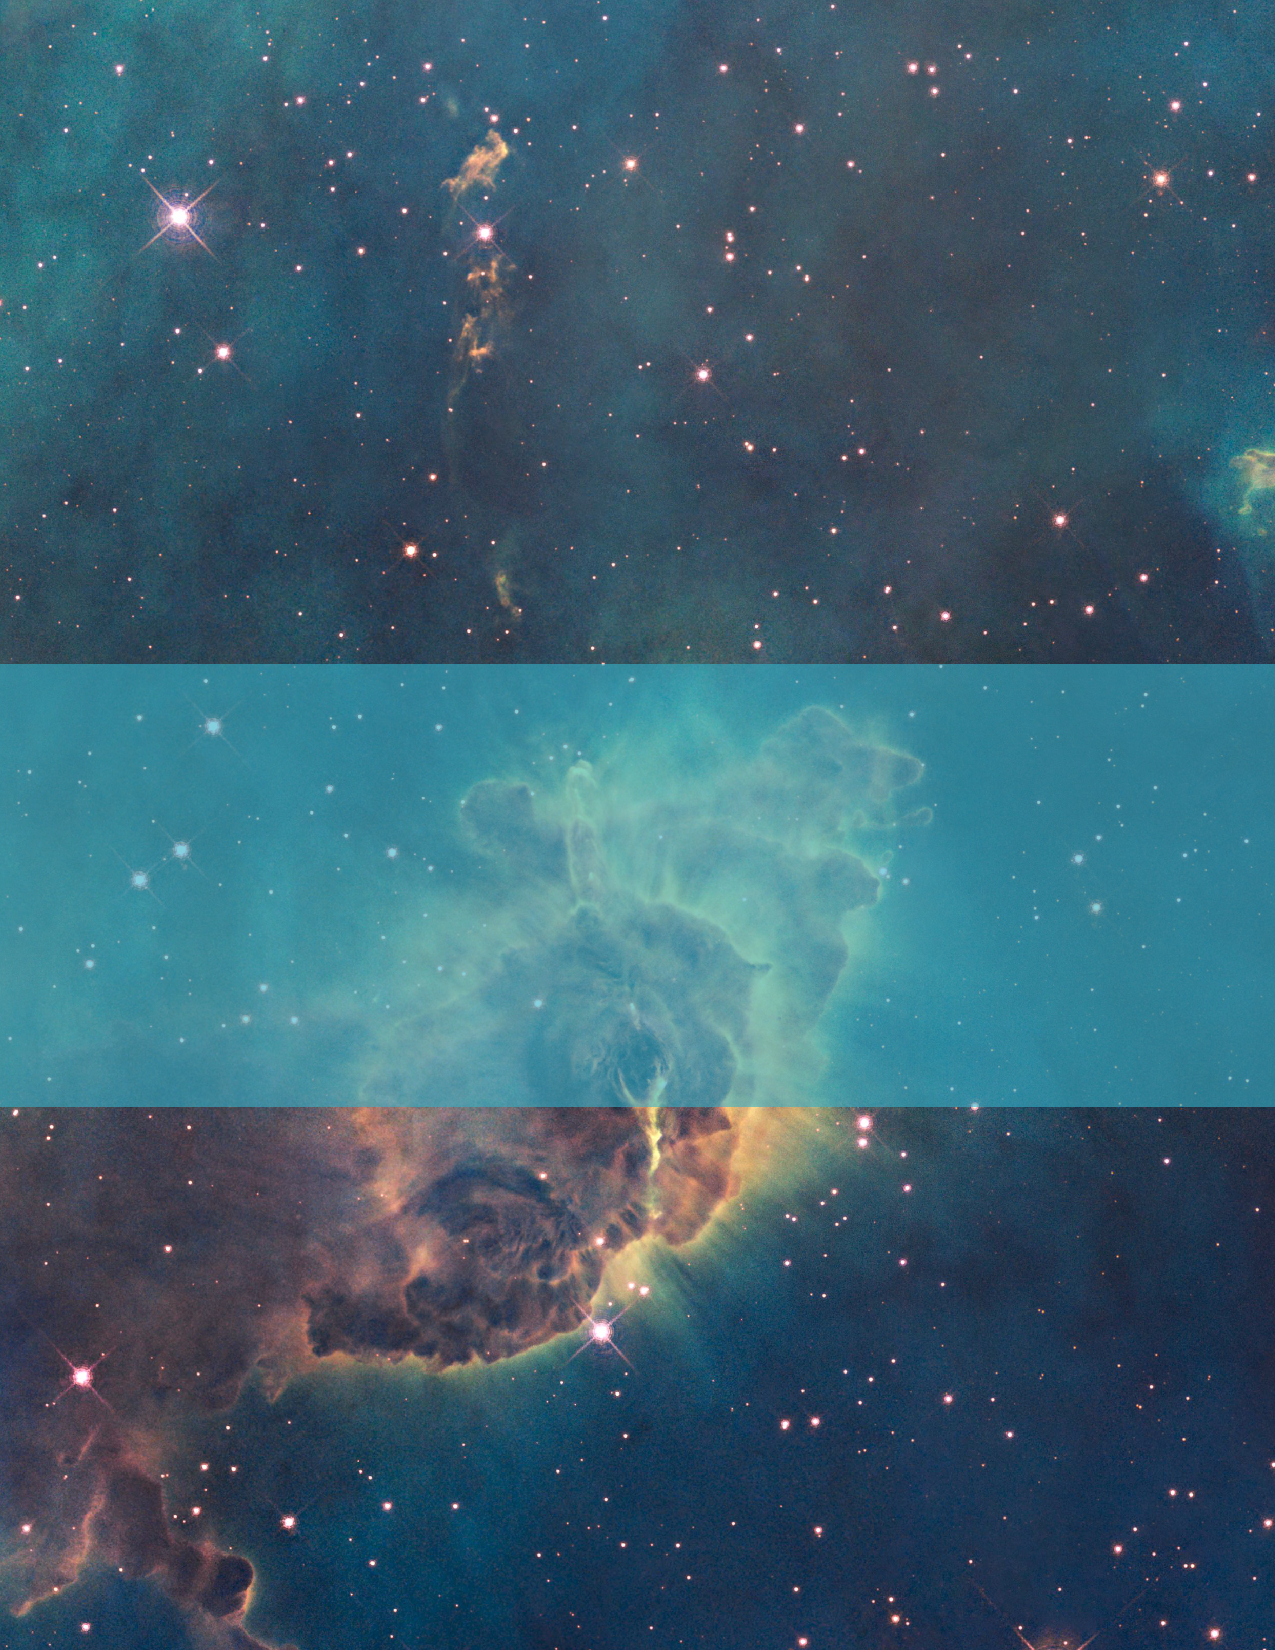
\includegraphics[scale=1.25]{esahubble}}} % Image background
\centering
\vspace*{5cm}
\par\normalfont\fontsize{35}{35}\sffamily\selectfont
\textbf{Calculus III}\\
{\LARGE github.com/mews6}\par % Book title
\vspace*{1cm}
{Jaime Torres}\par % Author name
\endgroup

%----------------------------------------------------------------------------------------
%	COPYRIGHT PAGE
%----------------------------------------------------------------------------------------

\newpage
~\vfill
\thispagestyle{empty}

%\noindent Copyright \copyright\ 2014 Andrea Hidalgo\\ % Copyright notice

\noindent \textit{First release, 2024} % Printing/edition date

%----------------------------------------------------------------------------------------
%	TABLE OF CONTENTS
%----------------------------------------------------------------------------------------

\chapterimage{head1.png} % Table of contents heading image

\pagestyle{empty} % No headers

\tableofcontents % Print the table of contents itself

%\cleardoublepage % Forces the first chapter to start on an odd page so it's on the right

\pagestyle{fancy} % Print headers again

%----------------------------------------------------------------------------------------
%	CHAPTER 1
%----------------------------------------------------------------------------------------

\chapterimage{head2.png} % Chapter heading image

\chapter{Introduction}

This is the persons i took the course with, they speak mostly spanish but they might help you!
\begin{itemize}
    \item Andres Angel (ja.angel908@uniandes.edu.co) 
    \item Hector Mora (hg.mora@uniandes.edu.co)   
\end{itemize}

\chapter{Linear Algebra Fundamentals}

In order to understand the concepts present in this module of calculus, a few preliminary concepts
in the realm of Linear Algebra are necessary, in order to not leave anybody lost, we'll be reviewing those topics.

\section{Vectors}
\subsection{Important operations}
\subsubsection{Addition and Subtraction}
Not much mystery to it, you can add and subtract the components in two different vectors:

\begin{gather*}
    \begin{pmatrix}
        x_1 \\ y_1 \\ z_1
    \end{pmatrix}
    +
    \begin{pmatrix}
        x_2 \\ y_2 \\ z_2
    \end{pmatrix} =
    \begin{pmatrix}
        x_1 + x_2 \\ y_1 + y_2 \\ z_1 + z_2
    \end{pmatrix} 
\end{gather*}

\subsubsection{Dot Product}

We can get a scalar product from the multiplication of the elements two vectors have
\begin{gather*}
    \begin{pmatrix}
        x_1 \\ y_1 \\ z_1
    \end{pmatrix}
    \cdot
    \begin{pmatrix}
        x_2 \\ y_2 \\ z_2
    \end{pmatrix} = x_1 x_2 + y_1 y_2 + z_1 z_2
\end{gather*}

This can also be written as:

\begin{gather}
    <\vec{u}, \vec{v}>
\end{gather}

\paragraph{Properties}

\begin{itemize}
    \item Dot product is commutative: $\vec{u} \cdot \vec{v} = \vec{v} \cdot \vec{u}$ 
    \item $\vec{u} \cdot \vec{v} = 0 \impliedby \implies \vec{u} \perp \vec{v}$
    \item $\vec{u} \cdot \vec{v} = ||\vec{u}|| ||\vec{v}|| \cos{\theta}$
    \item Cauchy Schwartz inequality: $|\vec{u}\cdot\vec{v}| \leq ||\vec{u}|| ||\vec{v}||$
    \item $\vec{u} \cdot \vec{u} = ||u||^2$
\end{itemize}

\subsubsection{Cross product}

Another form to multiply vectors, while getting another vector, is the cross prudict which we define as:

\begin{gather*}
    \begin{pmatrix}
        x_1 \\ y_1 \\ z_1
    \end{pmatrix}
    x
    \begin{pmatrix}
        x_2 \\ y_2 \\ z_2
    \end{pmatrix} = \begin{pmatrix}
        y_1 z_2 -z_1 y_2 \\ - (x_1 z_2 - z_1 x_2) \\ x_1 y_2 - y_1 x_2
    \end{pmatrix}
\end{gather*}

This specific operation cannot be done in dimensions that exceed $\mathbb{R}^3$
and can't be considered formally the multiplication of two vectors when the system is managed in $\mathbb{R}^n | n > 4$.
This course, however, is mostly managed for systems at most in 3 dimensions, hyperplanes will probably be tangentially 
asked about depending on the professor, but i wouldn't count on it. 

\paragraph{Properties}

Cross product operations have a few specific things that can happen.

\begin{itemize}
    \item $$\vec{u} x \vec{v} = - \vec{v} x \vec{u}$$
    \item $$ \vec{u} x \vec{v} \perp \vec{u} \land \vec{u} x \vec{v} \perp \vec{v} $$
    \item $$\vec{v} x \vec{u} = 0 \implies \vec{u} // \vec{v}$$
    \item $$||\vec{u} x \vec{v}|| = Surface$$
\end{itemize}

\paragraph*{Example}

Calculate the plane equation that includes the points:

\begin{gather}
    \vec{P} = (2,0,0) \\
    \vec{Q} = (0,1,0) \\
    \vec{R} = (0,0,3)
\end{gather}

\textit{\textbf{Solution}}

First of all, we'll do a normal vector via the cross product.
First, we'll need two vectors $\vec{PQ}$ and $\vec{PR}$ via vector subtraction:

\begin{gather}
    \vec{PR} = \begin{pmatrix}
        0\\0\\3
    \end{pmatrix} - \begin{pmatrix}
        2\\0\\0
    \end{pmatrix} = \begin{pmatrix}
        -2\\0\\3
    \end{pmatrix}\\
    \vec{PQ} = \begin{pmatrix}
        0\\1\\0
    \end{pmatrix} - \begin{pmatrix}
        2\\0\\0
    \end{pmatrix} = \begin{pmatrix}
        -2\\1\\0
    \end{pmatrix}
\end{gather}

And now, we can generate a cross product for these two mathematical objects, this should give us a vector normal to both:

\begin{gather}
    \vec{PQ} x \vec{PR} = \begin{pmatrix}
        -2\\1\\0
    \end{pmatrix} x \begin{pmatrix}
        -2\\0\\3
    \end{pmatrix} = 
\end{gather}

\paragraph{Example 2}

Find the Area of the triangle generated by the points:

\begin{gather}
    \vec{P} = (2,0,0) \\
    \vec{Q} = (0,1,0) \\
    \vec{R} = (0,0,3)
\end{gather}

For this, we can use the property of cross products being able to calculate a surface area to assume the way we can calculate a triangle from it:

\begin{gather}
    A_\triangle = \frac{||\vec{pq}x\vec{pr}||}{2}
\end{gather}

As given by our last example, then:

\begin{gather}
    A_\triangle = \frac{||(3,6,2)||}{2} = \frac{\sqrt{3^2+6^2+2^2}}{2} = \frac{\sqrt{9+36+4}}{2} = \frac{7}{2} 
\end{gather}


\subsubsection{Projection}

A proyection is the vector that can be found from making 

\begin{gather}
    Proy_{\vec{u}}(\vec{v}) = \alpha \vec{u}
\end{gather}

This has the following properties:

\begin{itemize}
    \item $ \vec{v} - \alpha \vec{u} \perp \vec{u} $
    \item $ \frac{\vec{u} \cdot \vec{v}}{||\vec{u}||^2} = \alpha $
\end{itemize}

We can also imagine the projection as:

\begin{gather}
    Proy_{\vec{u}}(\vec{v}) = (\frac{\vec{u}\cdot\vec{v}}{||\vec{u}||^2})\vec{u}
\end{gather}

\paragraph*{Example}

Given:

\begin{gather}
    \vec{u} = x+y=3\\
    \vec{v} = x+y=1
\end{gather}

What is the distance between both lines?

\textit{\textbf{Solution}}

For this we can check for the smallest distance between points, and since they are perpendicular to each other:

\begin{gather}
    \min d (\vec{v}, \vec{u}) = d(\vec{v}, \vec{u})
\end{gather}
lets instantiate the lines in a moment in time where they are both crossing the x axis:

\begin{gather}
    P = (0,1) \\
    Q = (0,3)
\end{gather}


\subsection{Properties}
\begin{itemize}
    \item two vectors are parallel if one is a multiple of the other, such as:
    $$\vec{v} = d\vec{w} ; d \in \mathbb{R}$$
    \item The angle between two vectors can be defined as such:
    $$\vec{v}\cdot\vec{w}=||\vec{v}|| ||\vec{w}|| \cos{\theta}$$
    If this operation is 0, then the two vectors are orthogonal (parallel) to each other.
    \item The cross product of two vectors is perpendicular to both vectors that generated it.
\end{itemize}

\section{Lines}

A line is simply a mathematical object of the form $ y = mx + b $ that unites two points in the space we're using, through a straight path, where and b is the cutting point in x=0.
and m is $\tan{\alpha}$, or the slope of this line. We can imagine it as:

\begin{gather}
    m = \frac{y_1 - y_0}{x_1 - x_0} \\
\end{gather}

another equation of this object is, when working on $\mathbb{R}^2$
is defined as:

\begin{gather}
    ax + by = c
\end{gather}

The reason this sort of expression is so useful, is because this \textbf{is a general form.} In other words, we can define with this system every single possible line in $\mathbb{R^2}$.
For example, let's imagine a line that is perfectly vertical. Such as it can be explained, intuitively, as $x = 1$:

%Image 1

This vector can't be expressed through formula 1,1 or y = mx + b, because it wouldn't cross the '0' axis, and it would have an infinite slope. But if we arrange it through (1,2), we can say:

\begin{gather}
ax + by = c\\
by = c - ax\\
y = \frac{c}{b} + \frac{a}{b} x
\end{gather}


We can suppouse $\frac{c}{b}$ as the cutting point with y, and then imagine $\frac{a}{b}$ as 'm', we can then, use an example where we set 'b' to be 0
and define a situation where x = 1.

\subsection{Lines in $\mathbb{R}^n$}

We can define lines in more dimensions than $\mathbb{R}^2$
through different forms. For example, we can imagine it as a parametric equation of the form:

\begin{gather}
    p = t\vec{v}
\end{gather}

\paragraph*{Example 2.2.1}

Find the parametric equation that passes through p = (1,2,3) and is parallel to the vector (1,0,-1)

\textit{\textbf{Solution}}
\begin{gather}
    \begin{pmatrix}
        1 \\ 2 \\ 3
    \end{pmatrix} + t \begin{pmatrix}
        1 \\0 \\-1
    \end{pmatrix}
\end{gather}

With this form, we can imagine that the solution actually is producing 3 different equations, and every single one defines how this object will behave in a different dimension.

therefore:

\begin{gather}
    x(t) = 1 + t \\ 
    y(t) = 2 \\
    z(t) = 3-t
\end{gather}

Pretty neat, huh?

We can define such an equation in 'n' dimensions that can define a line going through be it a plane or a hyperplane like this. We only need two vectors of the same 'n' dimension.
So, taking this form, can we express it in other ways? Well, yeah! ...and we just did. The before introduced equations can be called \textbf{the parametric equation of a line.}
the equation we generated


From here, we can also imagine that instead of using such a form, we can also equate everything to 't' and from here, we'll start defining a \textbf{Symetrical form of the line.}

In the previous example, we can imagine:
\begin{gather}
    x - 1 = y - 2 = \frac{z-3}{-1} = t    
\end{gather}

\section{Planes}

The plane can be defined as:

\begin{gather}
    ax + by + cz = d
\end{gather}

This plane can be defined with a point and a vector, for example:

\paragraph*{Example 2.3.1}
given $\vec{PQ} = (x,y,z)$ and $\vec{R} = (a,b,c)$, define a plane.

\textit{\textbf{Solution}}

\begin{gather}
    \begin{pmatrix}
        x - x_0 \\ y = y_0 \\ z - z_0
    \end{pmatrix} \cdot \begin{pmatrix}
        a\\b\\c
    \end{pmatrix} = 0\\
    a(x - x_0) + b(y - y_0) + c(z - z_0) = 0 \\
    ax - ax_0 + by - by_0 + cz - cz_0 = 0 \\
    ax + by + cz = ax_0 + by_0 + cz_0\\
    <d = ax_0 + by_0 + cz_0> \\
    ax + by + cz = d
\end{gather}

And from there we can define basically every plane in $\mathbb{R}^3$, as you can see, we arrived to the way we defined a plane in this dimension, and we could in theory, decide in a random point, a random vector, and start working from there into defining a plane.
But now, can we define a parametric equation of a plane, as we did with a line?

Well, the answer is yes.

the parametric form of a plane is actually pretty simple, as it is supremely similar to 
the one that defines a line, and is defined as:
\begin{gather}
    p + s\vec{v_1} + t \vec{v_2}
\end{gather}

if we generalize this into a system where R = (1,2,3), $v_1$ = (1,0,1) and $v_2$ = (1,1,0)
we can do a little example, written as:

\begin{gather}
    \begin{pmatrix}
        1\\2\\3
    \end{pmatrix} + s \begin{pmatrix}
        1\\0\\-1
    \end{pmatrix} + t\begin{pmatrix}
        1\\1\\0
    \end{pmatrix}
\end{gather}

\paragraph{Example 2.3.2}

Determine if the line 
\begin{gather}
    x = 9+5t\\
    y = -3+t\\
    z= 4t
\end{gather}

Intersects with the plane

\begin{gather}
    3x + 10y -2z+ 53
\end{gather}

If so, determine where.

\textit{\textbf{Solution}}

We can begin by replacing. Remember the line's equation and how it has x, y and z values.
\textbf{These values are equivalent to x, y and z in a plane}, and how you can replace it
in the plane's equation.

If we can solve the equation for
't', that means we can intersect that line with the 
plane and that it will intersect in that specific 't' point

\begin{gather}
    3(9 + 5t) + 10 (-3 + t) -2(4t) =53\\
    27 + 15t -30 + 10t -8t = 53\\
    t = \frac{56}{16} 
\end{gather}

\subsection*{Plane from 3 points in the space}

\paragraph{Example 2.3.3}

Find the line normal to the plane that crosses the points:
\begin{gather}
    P = (0,-3,-3)\\
    Q = (-3,0,-3)\\
    R = (-3,3,0)
\end{gather}

\textit{\textbf{Solution}}
We'll begin by getting two vectors from these lines, we can get them by subtracting one point from the other:
\begin{gather}
    \vec{PQ} = (-3,3,0)\\
    \vec{QR} = (0,-3,3)
\end{gather}

And now, we'll make a cross product between the two, so we can get a normal vector:

\begin{gather}
    \vec{PQ} x \vec{QR} = \begin{pmatrix}
        -3\\3\\0
    \end{pmatrix} x \begin{pmatrix}
        0\\-3\\3
    \end{pmatrix} = \begin{pmatrix}
        9\\9\\9
    \end{pmatrix} = \vec{n}
\end{gather}

Now, we can get from that normal vector, the direction vector for the line:

\begin{gather}
    \begin{pmatrix}
        x\\y\\z
    \end{pmatrix} = 
    \begin{pmatrix}
        0\\-3\\-3
    \end{pmatrix} + t\begin{pmatrix}
        9\\9\\9
    \end{pmatrix}
\end{gather}


\chapter{Non-Linear Fundamentals}
\section{Polar and Cylindrical Coordinates}

During the course, we'll be managing non-linear systems and such 
systems will require managing reference systems that are non-cartesian.
When trying to define parts of a line in algebra, we'll usually be looking at
coordinates, be them polar or cartesian. In either case, their information can be 
converted to the other system through the following formulas.

\begin{gather}
    \begin{cases}
        \rho = \sqrt{x^2+y^2} \\
        \theta = \arctan(\frac{y}{x})
    \end{cases}
    \text{\textit{cartesian to polar}}\\
    \begin{cases}
        \alpha_x = \rho \cos \theta \\
        \alpha_y = \rho \sin \theta
    \end{cases}
    \text{\textit{polar to cartesian}}
\end{gather}

Cartesian coordinates generally translate well to other dimensional spaces, such as would be the case
for $ \mathbb{R}^3 $, however, polar coordinates as we know them usually aren't as translatable in a direct
manner, and expressing them in three-dimensional spaces might be better suited to 
be expressed on a cylindrical or spherical condition. 
\subsection{Cylindrical coordinates}
In the case of cylindrical coordinates, the translation is probably the most intuitive, by computing
a cylinder with polar coordinates that indicate an (x,y) position, and a 'Z' variable indicating height 
that allows us to project the vector on a third dimension, this 'z' variable is exactly the same as it would be
on a cartesian model. We can express it like such:

$ \vec{v} = ( \rho, \theta, Z) $

conversion to a cartesian model can be expressed as:

\begin{gather}
    \vec(\alpha) =
    \begin{cases}
        \alpha_x = \rho \cos \theta \\
        \alpha_y = \rho \sin \theta \\
        \alpha_z = Z
    \end{cases}
    \text{\textit{Cylindrical to cartesian}}
    \\
    \vec(\alpha) =
    \begin{cases}
        \rho = \sqrt{x^2 + y^2} \\
        \theta =  \arctan(\frac{y}{x}) \\
        Z = Z
    \end{cases}
    \text{\textit{Cartesian to Cylindrical}}
\end{gather}

These coordinates might be useful to visualize circular 
functions, such as curves that take a cyllindrical, spring-like form.



\subsection{Spherical coordinates}

A spherical coordinate is formed by a tuple:

\begin{gather}
    (\rho, \theta ,\phi);
    \begin{cases}
        \rho \geq  0 \\
        0 \le \theta \le 2\pi \\
        0 \le \phi \le \pi    
    \end{cases}
\end{gather}

Where $ \rho $ is the magnitude of the vector, $\theta$ is the (x,y) coordinates, and
$\phi$ is the (y,z) angle. They must adhere to the following for it to be geometrically coherent:

\begin{equation}
    \begin{cases}
        \rho > 0 \\
        0 \le \phi \le \pi \\
        0 \le \theta \le 2\pi
    \end{cases}
\end{equation}

this tuple can generate two vectors:
\begin{equation}
    \begin{cases}
        \rho \sin \phi\\
        \rho
    \end{cases}
\end{equation}

And can be converted to a cartesian model as such:

\begin{gather}
    \vec(\alpha) =
    \begin{cases}
        \alpha_x = \rho \sin \phi \cos \theta \\
        \alpha_y = \rho \sin \phi \sin \theta \\
        \alpha_z = \rho \cos \phi
    \end{cases}
    \text{\textit{Spherical to cartesian}} \\ 
    \vec(\alpha) =
    \begin{cases}
        \rho = \sqrt{x^2 + y^2 + z^2} \\
        \theta =  \arctan(\frac{y}{x}) \\
        \phi = \arccos(\frac{z}{\sqrt{x^2+y^2+z^2}})
    \end{cases}
    \text{\textit{Cartesian to Spherical}}
\end{gather}

These are, of course, pretty useful to visualize spherical objects, but conic objects can also be easily expressed with this reference system.

\section{Scalar Functions}

For this course, there are moments in which we might manage more than a single variable on a single mathematical expression. 
We can imagine that there are functions can be defined as: 

\begin{gather}
    f(x_1, \dots, x_n) \underbrace{U}_{Domain} : \mathbb{R}^n \to \mathbb{R}
\end{gather}

This basically means, they project from a specific dimension to a point in $\mathbb{R}$.

Examples for this sort of function in $\mathbb{R}^2$ include:

\begin{gather}
    f(x,y) = x+y \\
    f(x,y) = x^2 + y^2 \\
    f(x,y) = e^{x^2y + y}
\end{gather}

We're going to like $\mathbb{R}^2 $ expressions on this course because they allow us to think of those functions in terms of a graphical representation on $\mathbb{R}^3$.
z will depend on both variables. We write this formally as:

\begin{gather}
    \{ (x,y,z) \in \mathbb{R}^3 | z = f(x,y) \}
\end{gather}


\section{Surface Curves}

A surface curve, as defined for $\mathbb{R}^3$, can be defined as sets of the form:

\begin{gather}
    \{ (x,y) \in \mathbb{R}^2 | f(x,y) = constant \}
\end{gather}

A surface curve can be defined with the value 'k' as:

\begin{gather}
    \{ (x,y) \in \mathbb{R}^2 | f(x,y) = k \}
\end{gather}

generally, we can say for the definition of these level curves:

\begin{itemize}
    \item If k < 0, there's no solution
    \item If k = 0, then it's a point
    \item If k>0, it's an elyptic form
\end{itemize}


\paragraph{Example 3.3.1}

Find the curves of $ f(x,y) = 1-x-y $

\textit{\textbf{Solution}}

\begin{gather}
    1 - k = x+y \ \text{Lines in $\mathbb{R^2}$}
\end{gather}

\subsection*{Intersection of a Surface with a plane}

We can make a surface intersect with a plane by replacing ont of the variables for the plane with 

\paragraph*{Example}

for $f(x,y) = x^2 + y^2$ make an intersection with $x^2 + y^2 = k $ 

\textit{\textbf{Solution}}

For this, we can think on the function as circles centered on the origin, whose radius will be 'k'.
Now, we can decide that 'x = 0' and we can try and check for values on which this is true for both expressions. This

\section{Limits and Continuity}

\subsection{Limits}

For this course, limits will be a fairly important mathematical operation. We
can imagine that limits can be described as:

\begin{gather}
    \lim_{x \to x_0} = L \implies \forall_{\epsilon > 0} \exists \delta > 0 \ if \ 0 < |x-x_0| < \delta \implies |f(x) - L| < \epsilon
\end{gather}

This means that for every number $\epsilon > 0$, there exists a $\delta >0$.
this will allow us to define ranges on which a function exists. epsilon and delta are but 
mathematical definitions of vertical and horizontal values for us to make a limit valid or invalid.

this definition is valid for limits with a single component, for multiple variables, we can assume:

\begin{gather}
    \lim_{x \to x_0} = L \implies \forall_{\epsilon > 0} \exists \delta > 0 \ if \ 0 < ||(x,y) - (x_0, y_0)|| < \delta \implies |f(x,y) - L| < \epsilon
\end{gather}

There are cases in which a limit exists and some others for which it doesn't. 

$$\lim f(x,y) \to L \implies (x,y) \to (a,b)$$

A limit doesn't exist if there is two ways of approaching the same point
for which the value of the limit is different. This can be seen when 


\paragraph{Example}

Solve:

$$\frac{xy}{x^2 + y^2}$$

\textit{\textbf{Solution}}

If we try to separate the values, we might get this

\begin{gather}
    \lim_{x \to 0} \frac{x \cdot 0}{x^2 + 0^2} = \lim_{x \to x_0} \frac{0}{x^2} = 0\\
    \lim_{y \to 0} \frac{y \cdot 0}{0^2 + y^2} = \lim_{y \to y_0} \frac{0}{y^2} = 0
\end{gather}

It would appear as if the limit existed,
but if we take them as a line of the form x=y, then we might get:

\begin{gather}
    \lim_{x \to 0} \frac{x \cdot x}{x^2 + x^2} = \lim_{x \to 0} \frac{x^2}{2x^2} = \frac{1}{2}  
\end{gather}

This doesn't exist, because 0 is different to $\frac{1}{2}$

Given the last example, how can we approach a function on infinite ways?
for this, we can imagine a line $ y = mx $ that can generalize all the possible lines in the plane. However, this can
also be done as explained in section 3.4.1, where we can establish a conversion to polar coordinates that will help our calculations.

\paragraph{Example}

Determine if the following limit exists:

$$\lim_{(x,y)\to(0,0)} \frac{y^4}{x^4+3y^4}$$

\textit{\textbf{Solution}}

\begin{gather}
<Y \ AXIS>\\
    \lim_{y \to 0} \frac{y^4}{3y^4}\\
    \lim_{y \to 0} \frac{1}{3}
\end{gather}

So the limit approaches $\frac{1}{3}$ when the value approaches zero

\begin{gather}
    <X \ AXIS>\\
    \lim_{x \to 0} \frac{0}{x^4} = \lim_{x\to 0} 0 = 0    
\end{gather}

You can approach the point from two different places when doing these limits, 
Therefore the limit DOES NOT EXIST. The limit is going to approach two different points


\subsection{Polar Coordinates for limits}

You can use polar coordinates for making a limit in two variables into one that only uses one.
so for example, you could pass a limit as such:

\begin{gather}
    \lim_{(x,y) \to (0,0)} F(x,y) = \lim_{\rho \to 0} f(\rho \cos{\theta}, \rho \sin{\phi})
\end{gather}

Then, we can evaluate rho as a single coordinate. This will also allow us to say that a limit exists
with certainty. 

\paragraph{Example}

Determine if the following limit exists:

$$\lim_{(x,y)\to(0,0)} \frac{e^{x^2 + y^2} - 1}{x^2 + y^2}$$

\textit{\textbf{Solution}}

it doesn't exist, for it doesn't tend to the values we expected. This is a process that would've been a lot more tedious if we did the separation that we 
applied for our previous example.


\paragraph{Example}

evaluate the following limit in its polar form: $$\frac{x^2}{x^2+y^2}$$

\textit{\textbf{Solution}}

\begin{gather}
    \lim_{r \to 0} \frac{(r^2 \cos^2{\theta})}{r^2}\\
    \lim_{r \to 0} = \cos^2{\theta} 
\end{gather}

Since it depends on $\theta$, then the limit does not exist. This is because theta might vary to values different from
what we want. 

\subsubsection{The limits of polar coordinates as a method}

It is possible that some limits, especially but not uniquely those that have targets different to (0,0), might break when trying to 
evaluate them through polar coordinates. A limit might break under a bunch of circumstances. 

\subsection{Continuity}

a function $\mathbb{R} \to \mathbb{R}$ is continuous if:

\begin{itemize}
    \item f is defined in $x_0$
    \item $\lim_{x \to x_0} f(x)$ exists
    \item $ f(x_0) = \lim_{x \to x_0} f(x) $
\end{itemize}

And, on two variables this can be seen as:

\begin{itemize}
    \item f is defined in $(x_0, y_0)$
    \item $\lim_{(x,y) \to (X_0, y_0)} f(x,y)$ exists
    \item $ f(x_0,y_0) = \lim_{(x,y) \to (x_0, y_0)} f(x,y) $
\end{itemize}

You can generalize it to $\mathbb{R}^n$

\chapter{Derivation/Differentiation}

a function in a single variable can have every single point on a curve being approximated to
a line, called a tangent. This z = (x,y) line variable can be defined by partial derivatives, that
can be described as:
\begin{equation}
    z_x = \frac{D_z}{D_x} = \frac{D_f}{D_x} (x,y) = \lim_{h \to 0} = \frac{(x+h,y)-f(x,y)}{h} 
\end{equation}
\begin{equation}
    \frac{d_f}{d_y}(x,y) = \lim_{h \to 0} = \frac{(x,y+h)-f(x,y)}{h}
\end{equation}
Where 'h' is a real number that tends towards zero.

In a more inmediately relevant manner, we can assume an 'f' function is differentiable in a point $x_0$ when:

\begin{gather}
    \lim_{x \to x_0} \frac{f(x)- f(x_0)}{x - x_0} \ exists 
\end{gather}

this can also be written as:

\begin{gather}
    \lim_{h \to 0} \frac{f(x)- f(x_0)}{h} \ exists 
\end{gather}

this means that the existence of a limit helps us check for differentiability.

\section{Partial Derivatives}

let:

\begin{gather}
    f(x,y) \mathbb{R}^2 \to \mathbb{R}
\end{gather}

Then we can imagine a derivation in respect of a single term, this will mean we'll take any 
other value as a sort of constant, that we will end up treating as such.

We can notate a derivation of this kind as $$\frac{\partial f}{\partial x}$$

\paragraph{Example}

Generate the partial derivatives of the following function:

$$f(x,y) = \frac{e^{y^{2}}}{x^2+y^2}$$

\section{Tangent Planes}

The plane tangent to the graph of a function f(x,y) in a point $(x_0, y_0)$
follows the following equation:

$$z = f(x_0, y_0) + \frac{\partial f}{\partial x} (x_0, y_0) [x - x_0] + \frac{\partial f}{\partial y} (x_0, y_0) [y - y_0] $$

\paragraph{Example}

Find the tangent plane to the graph $$f(x,y) = \frac{e^{y^{2}}}{x^2+y^2}$$ in the point (2,1)

\textit{\textbf{Solution}}

From our example of partial derivatives, we can say:

\begin{gather}
    f(2,1) = \frac{e}{5}\\
    \frac{\partial f}{\partial x} (2,1) =  \frac{-4e}{25}\\
    \frac{\partial f}{\partial y} (2,1) =  \frac{8e}{25}
\end{gather}

Therefore, we can write this plane as:

\begin{gather}
    z = \frac{e}{5} + \frac{-4e}{25}(x - 2) + \frac{8e}{25}(y - 1)
\end{gather}

once expanded, it will translate to a plane when graphed.

\paragraph*{Note}

The normal vector to a tangent plane is $$\vec{n} = (\frac{\partial f}{\partial x} (x_0, y_0), \frac{\partial f}{\partial y} (x_0, y_0), -1)$$

In a similar fashion, the normal vector to a surface in a point is basically the same, defined as:

$$(\frac{\partial f}{\partial x} (x_0, y_0), \frac{\partial f}{\partial y} (x_0, y_0), -1)$$

\section{Gradients}

given $$f(x,y) : \mathbb{R}^2 \to \mathbb{R}$$

the gradient of f(x,y) is defined as:

$$\nabla f(x,y) = (\frac{\partial f}{\partial x} (x,y), \frac{\partial f}{\partial y} (x,y))$$

and we have to take into account that:

$$\nabla f(x,y): \mathbb{R}^2 \to \mathbb{R}$$

given all of this, if f(x,y) is differentiable in $(x_0, y_0)$, then we can assume:

\begin{gather}
    f(x,y) ; f(x_0, y_0) + \nabla f(x_0, y_0) \begin{pmatrix}
        x - x_0 \\ y - y_0
    \end{pmatrix}
\end{gather}

this is an approximation for most situations where this happens, however this can also be written in a more precise
way if we assume it as:

If f is differentiable in $(x_0, y_0)$ and $$\frac{\partial f}{\partial x} (x_0, y_0) , \frac{\partial f}{\partial y} (x_0, y_0)$$
exist. Then

\begin{gather}
    \lim_{(x,y) \to (x_0, y_0)} \frac{f(x,y) - (f(x_0, y_0) + \nabla f(x_0, y_0) \ \begin{pmatrix}
        x - x_0 \\ y - y_0
    \end{pmatrix})}{||(x,y) - (x_0, y_0)||}
\end{gather}

\subsection{Chain Rule}

When we have a derivative that is composed of two functions, we can then 
calculate the derivative such as:

\subsubsection{First chain rule case}

On our first case, given a composed function, we can say:

\begin{gather}
    F(g(x))' = f'(g(x))\cdot g'(x)\\ <\text{Also written as:}> \\
    \frac{d(f^og)}{dx} = \frac{df}{dx}(g(x)) \cdot \frac{dg}{dx}
\end{gather}

we can write also write the chain rule as:

\begin{gather}
    \frac{d(f(g(t)))}{dt} = \nabla f(g(t)) \cdot g'(t)
\end{gather}

\begin{gather}
    g: \mathbb{R}^2 \to \mathbb{R}\\
    f: \mathbb{R}^2 \to \mathbb{R}\\
    f^o g \mathbb{R} \to \mathbb{R}
\end{gather}

\subsubsection{Second chain rule case}

given $$f: \mathbb{R}^2 \to \mathbb{R} | g: \mathbb{R}^2 \to \mathbb{R}$$
we might have a situation where these two functions depend on two other variables u,v. Then:

\begin{gather}
    \frac{\partial f(x(u,v), y(u,v))}{\partial u} = \frac{\partial f}{\partial x} (f(x(u,v), y(u,v))) \cdot \frac{\partial f}{\partial u} (u,v) + \frac{\partial f}{\partial y} (f(x(u,v), y(u,v))) \cdot \frac{\partial f}{\partial u} (u,v)
\end{gather}

A consequence of this system is that the gradient of a function is perpendicular to a 
level curve of the shape we're analyzing. This can be written as:

\begin{gather}
    \nabla f(x,y) \perp curve f(x_0,y_0) 
\end{gather}

\paragraph{Example 4,3,1}

Calculate a line normal to $x^2 + 2y^2 = 3$ in (1,1)

\textit{\textbf{solution}}

With the gradient of the function, we can then assume it will work like this, given we're assuming that the point they gave us is in the shape:

\begin{gather}
    f(x,y) = x^2 + 2y^2\\
    \nabla f(x,y) = (2x, 4y)\\
    \nabla f(1,1) = (2,4)\\
    \begin{pmatrix}
        1\\1
    \end{pmatrix} + t \begin{pmatrix}
        2\\4
    \end{pmatrix}
\end{gather}


\paragraph{Example 4,3,2}

Find the normal line and the tangent plane to:

$$x^2+y^2+2z^2=4$$ in (1,1,1)

\textit{\textbf{solution}}

For the tangent plane:

\begin{gather}
    f(x,y,z) = x^2 +y^2 +2z^2\\
    \nabla f(x,y,z) = (2x,2y,4z)\\
    \nabla f(1,1,1) = (2,2,4)\\
    line = \begin{pmatrix}
        1\\1\\1
    \end{pmatrix} + t \begin{pmatrix}
        2\\2\\4
    \end{pmatrix}\\
    Plane = 2(x-1) + 2(y-1) + 4(z-1) = 0 \\
    2x+2y+4z = 8
\end{gather}

\section{Superior order derivatives}

much like there is a way to do multiple integrals, we can do multiple partial derivatives, such as:

\begin{gather}
    \frac{\partial f}{\partial x} (x,y),\frac{\partial f}{\partial y} (x,y) \\
    f_{yx} = \frac{\partial^2 f}{\partial y \partial x} = \frac{\partial}{\partial y} \frac{\partial}{\partial x} f
\end{gather}

\paragraph{Theorem}

if f(x,y) has second derivatives and they're continuous, then:

\begin{gather}
    \frac{\partial^2 f}{\partial y \partial x} = \frac{\partial^2 f}{\partial x \partial y}  
\end{gather}

\section{Directional Derivatives}

We can talk about a directional derivative for the function 'f' in the direction 'V' as:

\begin{gather}
    F_{\vec{v}} f(p) = \frac{\lim_{h \to 0} f(p+hv) - f(p)}{h}
\end{gather}

This is the infinitesimal exchange rate towards v of a function f in p.

Given we have the chain rule, we can rewrite this as:

\begin{gather}
    \frac{d}{df}(f(p+tv)) ; t = 0
\end{gather}

A directional derivative is given by:

\begin{equation}
    D_{\vec{u}}f(x_0,y_0) = \frac{d}{dt} f(x_0 + t u_1, y_0 + t u_2) ; t = 0
\end{equation}

And we say that if a derivative exists, then $||\vec{u}|| = 1$;
f depends on x and y, and x and y both depend on t, this can be seen mathematically as:

\begin{equation}
    \frac{df}{dx} f(x_0 + t u_1, y_0 + t u_2) \underbrace{U_1}_{\frac{dx}{dt}} + \frac{df}{dy}(x_0 + t u_1, y_0 + t u_2) \underbrace{U_2}_{\frac{dy}{dt}}
\end{equation}

from this we can observe
\begin{equation}
    D_{\vec{u}}\ f(x_0, y_0) = \vec{\Delta} f(x_0, y_0) \centerdot \vec{u} = ||\vec{\Delta} f(x_0,y_0)|| \centerdot ||\vec{u}|| \centerdot \cos \theta\\
\end{equation}

So, given this set of conditions:

\begin{gather}
    \begin{cases}
        D_{\vec{u}} f(x_0, y_0) \text{  is maximal if $ \theta $ is 0} \\
        D_{\vec{u}} f(x_0, y_0) \text{  is minimal if $ \theta $ is $\pi$}
    \end{cases}
\end{gather}

We can infer then, regarding our direction:

\begin{equation}
    \vec{u} = \frac{\vec{\Delta} f(x_0, y_0)}{||\vec{\Delta}f(x_0,y_0)||}
\end{equation}

will make the function grow faster, and:

\begin{equation}
    \vec{u} = - \frac{\vec{\Delta} f(x_0, y_0)}{||\vec{\Delta}f(x_0,y_0)||}
\end{equation}

will make it decrease faster.

\subsubsection{Gradient Theorem}

If we describe formally our previous statements, we can find the gradient theorem.
this can be written as:

Given $$f(x,y,z): \mathbb{R}^3 \to \mathbb{{R}}$$
and a point $$P \in \mathbb{R}^3$$, we can say:

\begin{itemize}
    \item the fastest increasing direction of 'f' in 'P' is $$\vec{v} = \nabla f(p)$$
    \item the fastest decreasing direction of 'f' in 'P' is $$\vec{v} = - \nabla f(p)$$
\end{itemize}

\paragraph{Note}
\begin{gather}
    F_{\vec{v}} f(p) = \nabla f(p) \cdot \frac{\nabla f(p)}{||\nabla f(p)||} = ||\nabla f(p)||
\end{gather}

\paragraph{Example 1}

Temperature in a room is measured through the function $$T(x,y,z) = x^2 + 3y^2 + 2z^3$$

in the point (1,0,1), what is the fastest decreasing option?

\textbf{\textit{Solution}}

\begin{gather}
    \nabla T(x,y,z) = (2x,6y,6z^2)\\
    \nabla T(1,0,1) = (2,0,6)\\
    \vec{v} = - \nabla T(1,0,1) = -(2,0,6)
\end{gather}

\textit{Optional, normalize the vector}

\begin{gather}
    \frac{\vec{v}}{||\vec{v}||} = (\frac{-2}{2 \sqrt{10}}, 0, \frac{-6}{2\sqrt{10}})
\end{gather}

\paragraph{Example 1,1}

A person moves with a speed of $2 \frac{m}{s}$ through the room, what is the variation of temperature the person experiences?

\textbf{\textit{Solution}}

The minimum rate is:
\begin{gather}
    -||\nabla T(1,0,1)|| = - \sqrt{40} = -2\sqrt{10} \frac{{}^oC}{m}
    Var_{\frac{{}^oC}{S}} = Var_{\frac{{}^oC}{m}} \cdot (2 \frac{m}{s})\\
    (-2 \sqrt{10}\frac{{}^oC}{m}) \cdot (2 \frac{m}{s})
\end{gather}

\subsection{implicit equations}

An implicit surface equation given by $F(x,y,z) = C$ we can define, as a curve:

\begin{gather}
    \vec{r}t = <x(t),y(t),z(t)> \\
    \vec{r}t' = <x'(t),y'(t),z'(t)> 
\end{gather}

And from there we can assume that this curve is a part of S if:

\begin{gather}
    F(x(t), y(y), z(t)) = C ; \forall t
\end{gather}

Given this, F depends on x,y, and z and those three variables depend on t, allowing us
to affirm:

\begin{gather}
    F_x \frac{dx}{dt} + F_y \frac{dy}{dt} + F_z \frac{dz}{dt} \\
    \vec{\Delta} f \centerdot \vec{r}t' = 0
\end{gather}

geometrically this means the gradient is perpendicular to the tangent and therefore, the tangent plane.
to S in $(x_0,y_0,z_0)$, which can be expressed vectorially (and therefore, more usefully) as:

\begin{equation}
    \vec{\Delta}F(x_0,y_0,z_0) \centerdot \begin{pmatrix}
        x - x_0 \\ 
        y - y_0 \\ 
        z - z_0
    \end{pmatrix} = 0
\end{equation}

The line normal to S in $(x_0,y_0,z_0)$ can be defined as:

\begin{equation}
    \vec{n}(t) = \vec{x_0} + t\vec{\Delta} F(x_0,y_0,z_0)
\end{equation}

\begin{gather}
    D_{\vec{v}} f(p) = \nabla f(p) \cdot \vec{v} = ||\nabla f(p)|| \cdot ||\vec{v}|| \cos{\theta}
\end{gather}

\section{Theorems}

\paragraph{Theorem 8}

If f(x,y) is differentiable in $(x_0, y_0)$ then $f(x,y)$ is continuous in
$(x_0,y_0)$

\paragraph{Theorem 9}

if $f(x,y)$ has continual partial derivatives in $(x_0, y_0)$, then $f(x,y)$
is differentiable in $(x_0,y_0)$

\chapter{Optimization}

\section{Global Optimization}

\section{Optimization with equality restrictions}

We can restrict the range of a function to find the local minimum and maximum points in 
a specific set. 

For example let a function we're optimizing, that we'll call an objective function:
$$x^2 + y^2 -x+y$$ And we'll have a restriction we call the factible set, such as $$x^2+y^2=1$$.

Since $x^2+y^2-x+y$ is continuous in the set $x^2+y^2=1$ and the set
$x^2+y^2=1$ is closed and bound, for the extreme value theorem the problem has a solution.

\section{Lagrange Multipliers}
If f(x,y); g(x,y) are differentiable, such as we have $(x_0,y_0)$ that are maximum or minimum
of f(x,y) when bound to g(x,y) = C, then if $\nabla g(x_0, y_0) \neq \vec{0}$ , it means there exists a $\lambda \in \mathbb{R}$

We can write this as:

\begin{gather}
    \nabla f(x_0,y_0) = \lambda \nabla g(x_0, y_0)
\end{gather}


\end{document}